\documentclass[xcolor=pdflatex,dvipsnames,table]{beamer}
\usepackage{epsfig,graphicx}
\usepackage{palatino}
\usepackage{fancybox}
\usepackage{relsize}
\usepackage[procnames]{listings}
\usepackage{hyperref}
\usepackage{qtree} % needed?
\usepackage{booktabs}
\usepackage{dirtree}
\usepackage[normalem]{ulem}


% fatter TT font
\renewcommand*\ttdefault{txtt}
% another TT, suggested by Alex
% \usepackage{inconsolata}
% \usepackage[T1]{fontenc} % needed as well?


\newcommand{\scale}{0.7}

\newcommand{\todo}[1]{{\emph{TODO: #1}}}
\newcommand{\martin}[1]{{\color{blue} Martin: #1}}
\newcommand{\abcdef}[1]{{\color{red} Author2: #1}}

% uncomment following for final submission
%\renewcommand{\todo}[1]{}
%\renewcommand{\martin}[1]{}
%\renewcommand{\author2}[1]{}

\newcommand{\code}[1]{{\texttt{#1}}}

\hypersetup{
  linkcolor  = black,
%  citecolor  = blue,
  urlcolor   = blue,
  colorlinks = true,
}

\beamertemplatenavigationsymbolsempty
\setbeamertemplate{footline}[frame number]





\newif\ifbook
% shared in slides and book

\lstdefinelanguage{chisel}{
%  morekeywords={abstract,case,catch,class,def,%
%    do,else,extends,false,final,finally,%
%    for,if,implicit,import,match,mixin,%
%    new,null,object,override,package,%
%    private,protected,requires,return,sealed,%
%    super,this,throw,trait,true,try,%
%    type,val,var,while,with,yield},
%  otherkeywords={=>,<-,<\%,<:,>:,\#,@},
  sensitive=true,
  morecomment=[l]{//},
  morecomment=[n]{/*}{*/},
  morestring=[b]",
  morestring=[b]',
  morestring=[b]"""
}

\usepackage{color}
\definecolor{dkgreen}{rgb}{0,0.6,0}
\definecolor{gray}{rgb}{0.5,0.5,0.5}
\definecolor{mauve}{rgb}{0.58,0,0.82}

% Default settings for code listings
%\ifbook
\lstset{%frame=lines,
  language=chisel,
  aboveskip=3mm,
  belowskip=3mm,
  showstringspaces=false,
  columns=fixed, % basewidth=\mybasewidth,
  basicstyle={\small\ttfamily},
  numbers=none,
  numberstyle=\footnotesize,
  % identifierstyle=\color{red},
  breaklines=true,
  breakatwhitespace=true,
  procnamekeys={def, val, var, class, trait, object, extends},
  % procnamestyle=\ttfamily,
  tabsize=2,
  float
}
%\else
%\lstset{%frame=lines,
%  language=chisel,
%  aboveskip=3mm,
%  belowskip=3mm,
%  showstringspaces=false,
%  columns=fixed, % basewidth=\mybasewidth,
%  basicstyle={\small\ttfamily},
%  numbers=none,
%  numberstyle=\footnotesize\color{gray},
%  % identifierstyle=\color{red},
%  keywordstyle=\color{blue},
%  commentstyle=\color{dkgreen},
%  stringstyle=\color{mauve},
%  breaklines=true,
%  breakatwhitespace=true,
%  procnamekeys={def, val, var, class, trait, object, extends},
%  procnamestyle=\ttfamily\color{red},
%  tabsize=2,
%  float
%}
%\fi

\lstnewenvironment{chisel}[1][]
{\lstset{language=chisel,#1}}
{}

\newcommand{\shortlist}[1]{{\lstinputlisting[nolol]{#1}}}

\newcommand{\longlist}[3]{{\lstinputlisting[float, caption={#2}, label={#3}, frame=tb, captionpos=b]{#1}}}

\newcommand{\verylonglist}[3]{{\lstinputlisting[caption={#2}, label={#3}, frame=tb, captionpos=b]{#1}}}


\title{Refactor of State Machines}
\author{Martin Schoeberl}
\date{\today}
\institute{Technical University of Denmark\\
Embedded Systems Engineering}

\begin{document}

\begin{frame}
\titlepage
\end{frame}

\begin{frame}[fragile]{Outline}
\begin{itemize}
%\item TODO: Maybe more on display multiplexing
\item Today one hour lecture planned, but probably a bit longer
\item Repeat finite-state machine with datapath
\item Factoring of finite-state machines
\item Advanced Chisel: functions and parametrization
\item Talk on todays (and next week) lab exercise
\end{itemize}
\end{frame}

\begin{frame}[fragile]{Exam Info}
\begin{itemize}
\item Exam will be online at home
\item All aids allowed with open Internet
\item But DTU is very harsh on cheating, just don't do it
\item Multiple choice plus PDF with questions
\item Upload solution in a single PDF
\begin{itemize}
\item Please use your study number as file name
\item Train to do a drawing and integrate it into a PDF
\end{itemize}
\item Timing exercise, some coding, understanding questions, drawing circuits
\item We will do a test exam
\end{itemize}
\end{frame}

\begin{frame}[fragile]{A (Minimal) Project from Scratch}
\begin{itemize}
\item \emph{It is cumbersome to set up new Chisel project without a template.}
\item \emph{I would like if we were taught how to create our own programs in Chisel, instead of just filling out the necessary code in a program you have already created.}
\item Just two files: \code{build.sbt} and a \code{.scala} file
\item Create the folder/directory structure
\item Copy a \code{build.sbt}
\item Import in InteliJ
\item Create a \code{.scala} class
\item Show it now
\item Do this exercise today!
\end{itemize}
\end{frame}

\begin{frame}[fragile]{Workflow}
\begin{itemize}
\item \emph{It could be nice to hear more about how to best organize a project/workflow when you are multiple people working on the same project. Maybe some guiding principles and good practices that can be followed.}
\item Share code on GitHub (private repo)
\item Meet in Zoom: you all have a full license from DTU
\begin{itemize}
\item You can take over a screen to type
\item You can draw on it
\item Besides ad-hoc meetings, have a regular project meeting
\end{itemize}
\item Use Slack for quick notes and quick sharing of files
\item Maybe also try to share the \code{.bit} file for the FPGA board
\item Use Google docs for taking notes, start your report
\item If you like Latex, use overleaf
\end{itemize}
\end{frame}


%\begin{frame}[fragile]{Show Example on ``Whiteboard''}
%\end{frame}

\begin{frame}[fragile]{FSM with Datapath}
\begin{itemize}
\item A type of computing machine
\item Consists of a finite-state machine (FSM) and a datapath
\item The FSM is the master (the controller) of the datapath
\item The datapath has computing elements
\begin{itemize}
\item E.g., adder, incrementer, constants, multiplexers, ...
\end{itemize}
\item The datapath has storage elements (registers)
\begin{itemize}
\item E.g., sum of money payed, count of something, ...
\end{itemize}
\end{itemize}
\end{frame}

\begin{frame}[fragile]{FSM-Datapath Interaction}
\begin{itemize}
\item The FSM controls the datapath
\begin{itemize}
\item For example, add 2 to the sum
\end{itemize}
\item By controlling multiplexers
\begin{itemize}
\item For example, select how much to add
\item Not adding means selecting 0 to add
\end{itemize}
\item Which value goes where
\item The FSM logic also depends on datapath output
\begin{itemize}
\item Is there enough money payed to release a can of soda?
\end{itemize}
\item FSM and datapath interact
\end{itemize}
\end{frame}


\begin{frame}[fragile]{Popcount Example}
\begin{itemize}
\item An FSMD that computes the popcount
\item Also called the Hamming weight
\item Compute the number of `1's in a word
\item Input is the data word
\item Output is the count
\item Code available at \href{https://github.com/schoeberl/chisel-book/blob/master/src/main/scala/PopCount.scala}{PopCount.scala}
\end{itemize}
\end{frame}

\begin{frame}[fragile]{Popcount Block Diagram}

\begin{figure}
  \includegraphics[scale=\scale]{../figures/popcnt-fsmd}
\end{figure}
\end{frame}


\begin{frame}[fragile]{Popcount Connection}
\begin{columns}
\column{0.6\textwidth}
\begin{itemize}
\item Input \code{din} and output \code{popCount}
\item Both connected to the datapath
\item We need some handshaking
\item For data input and for count output
\end{itemize}
\column{0.4\textwidth}
\begin{figure}
  \includegraphics[scale=0.45]{../figures/popcnt-fsmd}
\end{figure}
\end{columns}
\end{frame}

\begin{frame}[fragile]{Popcount Handshake}
\begin{columns}
\column{0.6\textwidth}
\begin{itemize}
\item We use a ready-valid handshake
\item When data is available valid is asserted
\item When the receiver can accept data ready is asserted
\item Transfer takes place when both are asserted
\end{itemize}
\column{0.4\textwidth}
\begin{figure}
  \includegraphics[scale=0.45]{../figures/popcnt-fsmd}
\end{figure}
\end{columns}
\end{frame}


\begin{frame}[fragile]{The FSM}
\begin{figure}
  \includegraphics[scale=\scale]{../figures/popcnt-states}
\end{figure}
\begin{itemize}
\item A Very Simple FSM
\item Two transitions depend on input/output handshake
\item One transition on the datapath output
\end{itemize}
\end{frame}

\begin{frame}[fragile]{The Datapath}
\begin{figure}
  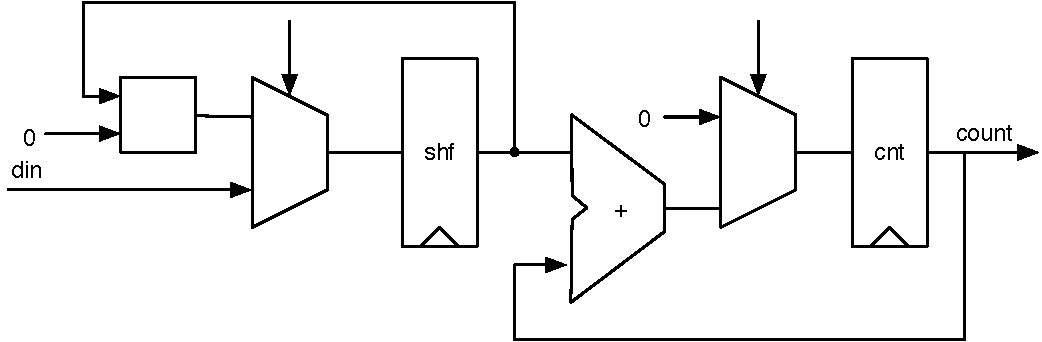
\includegraphics[scale=0.65]{../figures/popcnt-data}
\end{figure}
\end{frame}

\begin{frame}[fragile]{Let's Explore the Code}
\begin{itemize}
\item In \href{https://github.com/schoeberl/chisel-book/blob/master/src/main/scala/PopCount.scala}{PopCount.scala}
\end{itemize}
\end{frame}

\begin{frame}[fragile]{Usage of an FSMD}
\begin{itemize}
\item Maybe the main part your vending machine is an FSMD?
\end{itemize}
\end{frame}



\begin{frame}[fragile]{Factoring FSMs}
\begin{itemize}
\item Divide a big problem into several smaller problems
\item Splitting a FSM into two or more
\begin{itemize}
\item Simplify the design
\end{itemize}
\item FSMs communicate via logic signals
\begin{itemize}
\item FSM provides input controls signals to another
\item FSM senses output from another
\end{itemize}
\end{itemize}
\end{frame}

\begin{frame}[fragile]{Specification Of a Light Flasher}
\begin{itemize}
\item Inputs: \code{start}
\item Outputs: \code{light}
\item Operation:
\begin{itemize}
\item When in = 1, FSM goes through 5 sequences:
\begin{itemize}
\item On-Off-On-Off-On
\end{itemize}
\item Each On sequence (\code{flash}):
\begin{itemize}
\item out = 1
\item 6 cycles long
\end{itemize}
\item Each Off sequence (\code{space}):
\begin{itemize}
\item out = 0
\item 4 cycles long
\end{itemize}
\item After 5 sequences, FSM goes back to \code{off} state to wait for new input
\end{itemize}
\end{itemize}
\end{frame}

\begin{frame}[fragile]{Light Flasher State Diagram}
\begin{itemize}
\item Example from Dally, Chapter 17
\item Copyright figure, so show it from older slides
\end{itemize}
\end{frame}

\begin{frame}[fragile]{Specification Change}
\begin{itemize}
\item We have a flat FSM with 27 states
\begin{itemize}
\item 27 \code{is(state)} statements
\end{itemize}
\item If we change the specification to
\begin{itemize}
\item 12 cycles for each flash
\item 4 flashes
\item 7 cycles between flashes
\item Complete change of \code{switch} statement
\item Now 70 \code{is} statements!
\end{itemize}
\item This does not scale
\end{itemize}
\end{frame}

\begin{frame}[fragile]{Factor Light Flasher}
\begin{itemize}
\item Factor out counting on and off intervals
\begin{itemize}
\item Into a timer
\item Reduces 6 and 4 states sequences into two single states
\end{itemize}
\item Results in
\begin{itemize}
\item a master FSM and
\item a timer FSM
\end{itemize}
\item Simplifies FSMs
\item Allows easier change of interval lengths
\end{itemize}
\end{frame}


%\begin{frame}[fragile]{Working Break}
%\begin{itemize}
%\item Build your own ``camera'' stand
%\item 20 minutes
%\item Show your solution to the others at the end of the break
%\begin{itemize}
%\item Don't expose it too early ;-)
%\end{itemize}
%\end{itemize}
%\end{frame}

\begin{frame}[fragile]{Factored Light Flasher}
\begin{figure}
  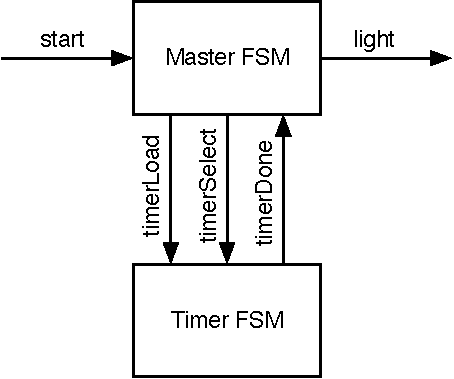
\includegraphics[scale=\scale]{../figures/flasher}
\end{figure}
\begin{itemize}
\item Time loads value 5 or 3, based in \code{timerSelect}
\end{itemize}
\end{frame}

\begin{frame}[fragile]{Timer Specification}
\begin{itemize}
\item Two inputs
\begin{itemize}
\item \code{timerLoad} to load the down counter
\item \code{timerSelect} to select between 6 and 4 cycles counting
\end{itemize}
\item Output
\begin{itemize}
\item \code{timerDone} is 1 when counter has completed the countdown
\item Remains asserted until counter reloaded
\end{itemize}
\item Counter can be (re)loaded in any state
\begin{itemize}
\item When not loaded it counts down to zero
\end{itemize}
\item Similar to the timer we looked at two weeks ago
\end{itemize}
\end{frame}

\begin{frame}[fragile]{The Timer FSM}
\shortlist{../code/flasher_timer.txt}
\end{frame}

\begin{frame}[fragile]{The Master FSM}
\begin{itemize}
\item Show in IntelliJ
\item Run test and show waveform
\end{itemize}
\end{frame}


%\begin{frame}[fragile]{State Diagram of Factored Light Flasher}
%\begin{itemize}
%\item yyy
%\end{itemize}
%\end{frame}
%
%\begin{frame}[fragile]{Waveforms from simulation of light-flasher FSM}
%\begin{itemize}
%\item yyy
%\end{itemize}
%\end{frame}

\begin{frame}[fragile]{Result of Refactoring}
\begin{itemize}
\item State of original flat FSM has been separated
\item The part of cycle counting in the counter
\item Part flash or space in master FSM
\item Represent original 27 states in just two 6 states FSMs
\item 
\item BTW: the master FSM is a Mealy FSM
\end{itemize}
\end{frame}

\begin{frame}[fragile]{Still Redundancy in FSM}
\begin{itemize}
\item \code{flash1}, \code{flash2}, and \code{flash3} same function
\item \code{space1} and \code{space2} same function
\item Refactor number of remaining flashes
\item Master FSM states: \code{off}, \code{flash},
and \code{space}
\end{itemize}
\end{frame}

\begin{frame}[fragile]{Factor out ``flash number''}
\begin{figure}
  \includegraphics[scale=\scale]{../figures/flasher2}
\end{figure}
\end{frame}

\begin{frame}[fragile]{Counter}
\shortlist{../code/flasher2_counter.txt}
\begin{itemize}
\item Loaded with 2 for 3 flashes
\item Counts the \emph{remaining} flashes
\end{itemize}
\end{frame}

\begin{frame}[fragile]{Code of Flasher2}
\begin{itemize}
\item Show in IntelliJ
\item Run test and show waveform
\end{itemize}
\end{frame}



%\begin{frame}[fragile]{State diagram of twice-factored light flasher}
%\begin{itemize}
%\item yyy
%\end{itemize}
%\end{frame}

\begin{frame}[fragile]{Benefits of Refactored Solution}
\begin{itemize}
\item Master FSM has just three states: \code{off}, \code{flash}, and \code{space}
\item Change of intervals or number of flashes needs no change in the FSM
\item Smaller components are easier to read and simpler to test individually
\end{itemize}
\end{frame}

\begin{frame}[fragile]{Usage in your VM}
\begin{itemize}
\item Maybe factor out the edge detection for the button(s)
\item Use a timer for more advanced user interface
\begin{itemize}
\item Blinking LED on some error
\item Write text as a banner in the 7-segment display
\item ...
\end{itemize}
\end{itemize}
\end{frame}

\begin{frame}[fragile]{Functions}
\begin{itemize}
\item Circuits can be encapsulated in functions
\item Each \emph{function call} generates hardware
\item A function is defined with \code{def} \emph{name}
\item Similar to a method in Java
\item Simple functions can be a single line
\end{itemize}
\begin{chisel}
  def adder(v1: UInt, v2: UInt) = v1 + v2
  
  val add1 = adder(a, b)
  val add2 = adder(c, d)
\end{chisel}
\end{frame}

\begin{frame}[fragile]{More Function Examples}
\begin{itemize}
\item Functions can also contain registers
\end{itemize}
\begin{chisel}
  def addSub(add: Bool, a: UInt, b: UInt) =
    Mux(add, a + b, a - b)

  val res = addSub(cond, a, b)

  def rising(d: Bool) = d && !RegNext(d)

  val edge = rising(cond)
\end{chisel}
\end{frame}

\begin{frame}[fragile]{The Counter as a Function}
\begin{itemize}
\item Longer functions in curly brackets
\item Last value is the return value
\end{itemize}
\begin{chisel}
def counter(n: UInt) = {
  
  val cntReg = RegInit(0.U(8.W))
  
  cntReg := cntReg + 1.U
  when(cntReg === n) {
    cntReg := 0.U
  }
  cntReg
}

val counter100 = counter(100.U)
\end{chisel}
\end{frame}

\begin{frame}[fragile]{Functional Abstraction}
\begin{itemize}
\item Functions for repeated pieces of logic
\item May contain state
\item Functions may return \emph{hardware}
\item More lightweight than a \code{Module}
\end{itemize}
\end{frame}

%\begin{frame}[fragile]{Functions}
%\begin{itemize}
%\item Example from Patmos execute stage
%\end{itemize}
%\begin{chisel}
%def alu(func: Bits, op1: UInt, op2: UInt): Bits = {
%  val result = UInt(width = DATA_WIDTH)
%  // some more lines...
%  switch(func) {
%    is(FUNC_ADD) { result := sum }
%    is(FUNC_SUB) { result := op1 - op2 }
%    is(FUNC_XOR) { result := (op1 ^ op2).toUInt }
%    // some more lines
%  }
%  result
%}
%\end{chisel}
%\end{frame}

\begin{frame}[fragile]{Parameterization}
\begin{chisel}
class ParamChannel(n: Int) extends Bundle {
  val data = Input(UInt(n.W))
  val ready = Output(Bool())
  val valid = Input(Bool())
}

val ch32 = new ParamChannel(32)
\end{chisel}
\begin{itemize}
\item Bundles and modules can be parametrized
\item Pass a parameter in the constructor
\end{itemize}

\end{frame}
\begin{frame}[fragile]{A Module with a Parameter}
\shortlist{../code/param_adder.txt}
\begin{itemize}
\item Parameter can also be a Chisel type
%\item Can also be a generic type:
%\item \code{class Mod[T <: Bits](param: T) extends...}
\end{itemize}
\end{frame}

\begin{frame}[fragile]{Use the Parameter}
\shortlist{../code/use_param_adder.txt}
\begin{itemize}
\item Can be used for the display multiplexing configuration
\end{itemize}
\end{frame}

\begin{frame}[fragile]{Today's Lab - Update below}
\begin{itemize}
\item Driving your 7-segment decoder
\item Use a counter to count from 0 to 15, driving your display
\item Use another counter to generate your timing
\begin{itemize}
\item We talked about this today
\end{itemize}
\item You clock on the board is 100 MHz
\item The given tester does only generate a waveform, no testing
\item Use a different maximum count value for waveform debugging
\item Then synthesize it for the FPGA
\item Show a TA your working design
\item \href{https://github.com/schoeberl/chisel-lab/tree/master/lab8}{Lab 8}
\end{itemize}
\end{frame}

\begin{frame}[fragile]{Today Lab}
\begin{itemize}
\item Do a project from scratch
\item Display multiplexing
\item Described in Vending Machine Specification (show)
\item This week and next week
\item Can also be developed in simulation
\end{itemize}
\end{frame}

\begin{frame}[fragile]{Display Multiplexing -- Move to next week}
\begin{itemize}
\item Saving of pins in the FPGA
\item Switch between the four digits at around 1 kHz
\item Switch \emph{faster} in simulation
\item Show code
\item Also includes a display simulation for those without an FPGA
\item \href{https://github.com/schoeberl/chisel-lab/tree/master/lab8}{Lab 8}
%\item Sketch needed hardware
\end{itemize}
\end{frame}



\begin{frame}[fragile]{Summary}
\begin{itemize}
\item Divide a bigger problem into smaller ones
\begin{itemize}
\item Easier to design
\item Easier to test
\item Sometimes only feasible solution
\end{itemize}
\item Factoring state machines
\begin{itemize}
\item Separate state into multiple `orthogonal' state variables
\item Each is simpler to handle (fewer states)
\item ``Factors out'' repetitive sequences
\item Hierarchical structure
\end{itemize}
\end{itemize}
\end{frame}




\end{document}

%\begin{frame}[fragile]{xxx}
%\begin{itemize}
%\item yyy
%\end{itemize}
%\end{frame}
